\documentclass[12pt]{article}
\usepackage{enumitem}
\usepackage{mathtools}
\usepackage{amsthm}
\usepackage{graphicx}
\graphicspath{ {images/} }
\begin{document}

\title{Assignment 10}
\author{Darwin Ding}
\maketitle

\section*{Exercise 6.1}
\begin{enumerate}[label=(\alph*)]
	\item Consider a circle centered on the origin. Put two points on the circle such that the line segment between them is a diameter of the circle. Each of these points represents a vector. Clearly, by cosine similarity, these points are as far apart as they could be, as the angle between the vectors is a full 180 degrees. However, as you shrink the radius of the circle the Euclidean distance will decrease more and more. After sufficient shrinkage, you'll be left with a situation where the two vectors are completely dissimilar by cosine similarity, but very similar by Euclidean distance.
	\\ \\ Consider two vectors with a single feature that differs by very little. Both cosine similarity and Euclidean distance will say these two vectors are the same. If you were to add additional features to both vectors that are identical to the feature already there, you would find that the cosine similarity would not change but the Euclidean distance would continue to get larger and larger. With sufficient features, Euclidean distance will say these vectors are very dissimilar but cosine similarity will not agree.
	\item Cosine similarity will change with changes in the origin. Euclidean distance is just the raw differences between all of the components of both vectors, so if the origin shifts all of the components will individually shift in the same way. However, cosine similarity is defined as the angular distance between two vectors, and if you change where the origin is, the vectors' angles from the origin will change.
	\\ \\ In general, cosine similarity would be the best metric to pick for the job. Euclidean distance is very fickle and implementation heavy, and naturally decreases with an increasing number of features because it's a simple sum.
\end{enumerate}

\section*{Exercise 6.2}
\begin{enumerate}[label=(\alph*)]
	\item If f(x) returns +1 (which will happen with probability $\pi(x)$, where $pi(x) \ge 0.5$) but the correct classification was -1, we've committed an error. Similarly, if we return -1 (which happens with probability $\pi(x)$, where $\pi(x) \le 0.5$) but the correct classification was +1, we've committed an error.
	
	The former case happens by definition with probability $1 - \pi(x) \le 0.5$, and the latter case happens by definition with probability $\pi(x) \le 0.5$. Because of the definition of f(x), we will always select the classification that $\pi(x)$ leans towards. One of $\pi(x)$ and $1 - \pi(x)$ will be less than 0.5 and the other will be greater, and so the error can only be the minimum of the two.
	\item This is by definition the best behavior we can have, because in each case we select the option that has the least probability of error. If we create any other hypothesis that disagrees on a certain point, we are by definition selecting the option that has the higher probability of error.
	
	For instance, if $\pi(x) < 0.5$ (if $\pi(x) = 0.5$ there isn't any real difference between which class we select), f(x) will output -1 and have an error with probability $\pi(x) < 0.5$. Any hypothesis that disagrees with this will output +1 and have an error of $1 - \pi(x) > 0.5$.
\end{enumerate}

\section*{Problem 6.1}
\begin{enumerate}[label=(\alph*)]
	\item The following graph is what the 1-NN decision boundaries look like for the data set. It is a little difficult to make out individual points, but the circles within the colored regions are the actual data points.
	
	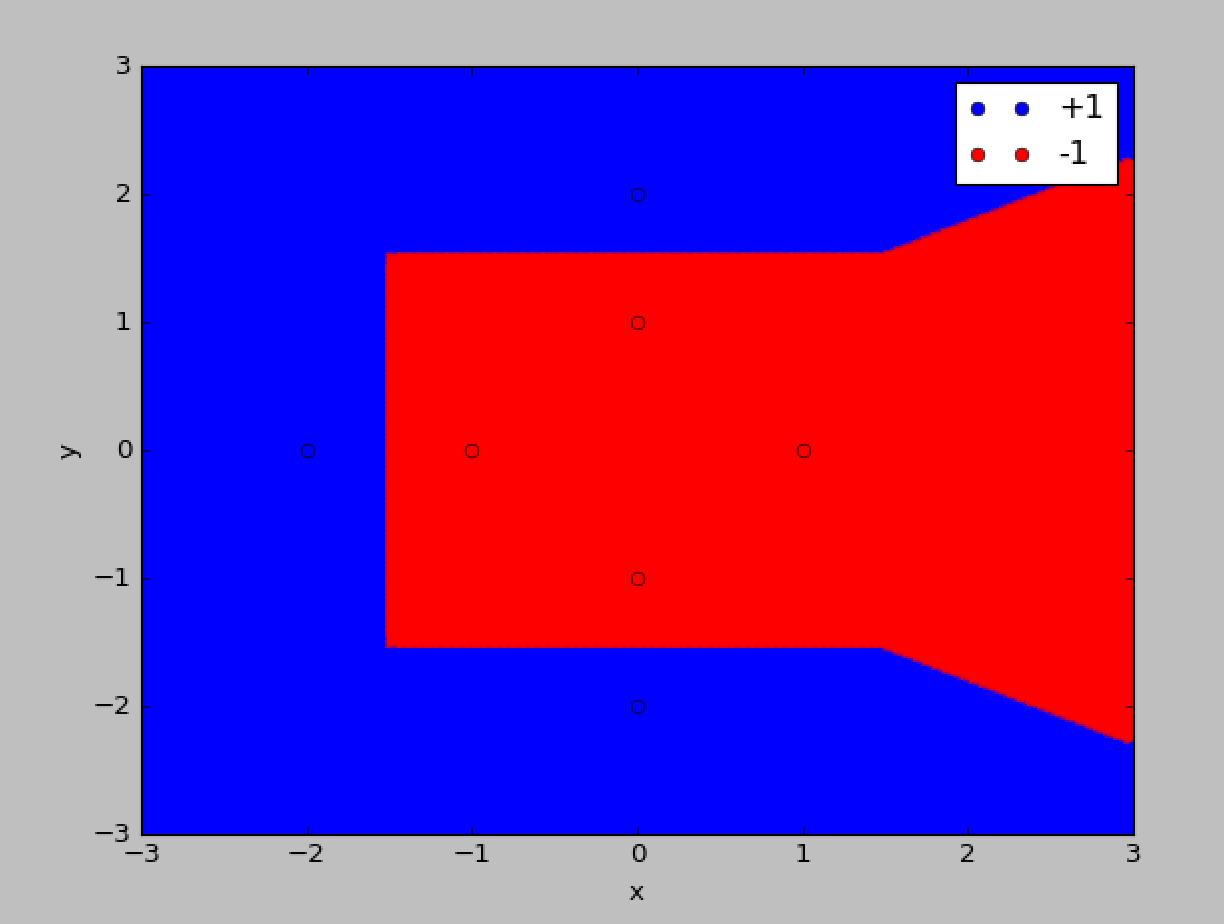
\includegraphics[scale=0.6]{6-1a1.png}
	
	Similarly, here is the graph for 3-NN decision boundaries. This may look somewhat surprising, but it occurs due to the blue +1 points being relatively far apart.
	
	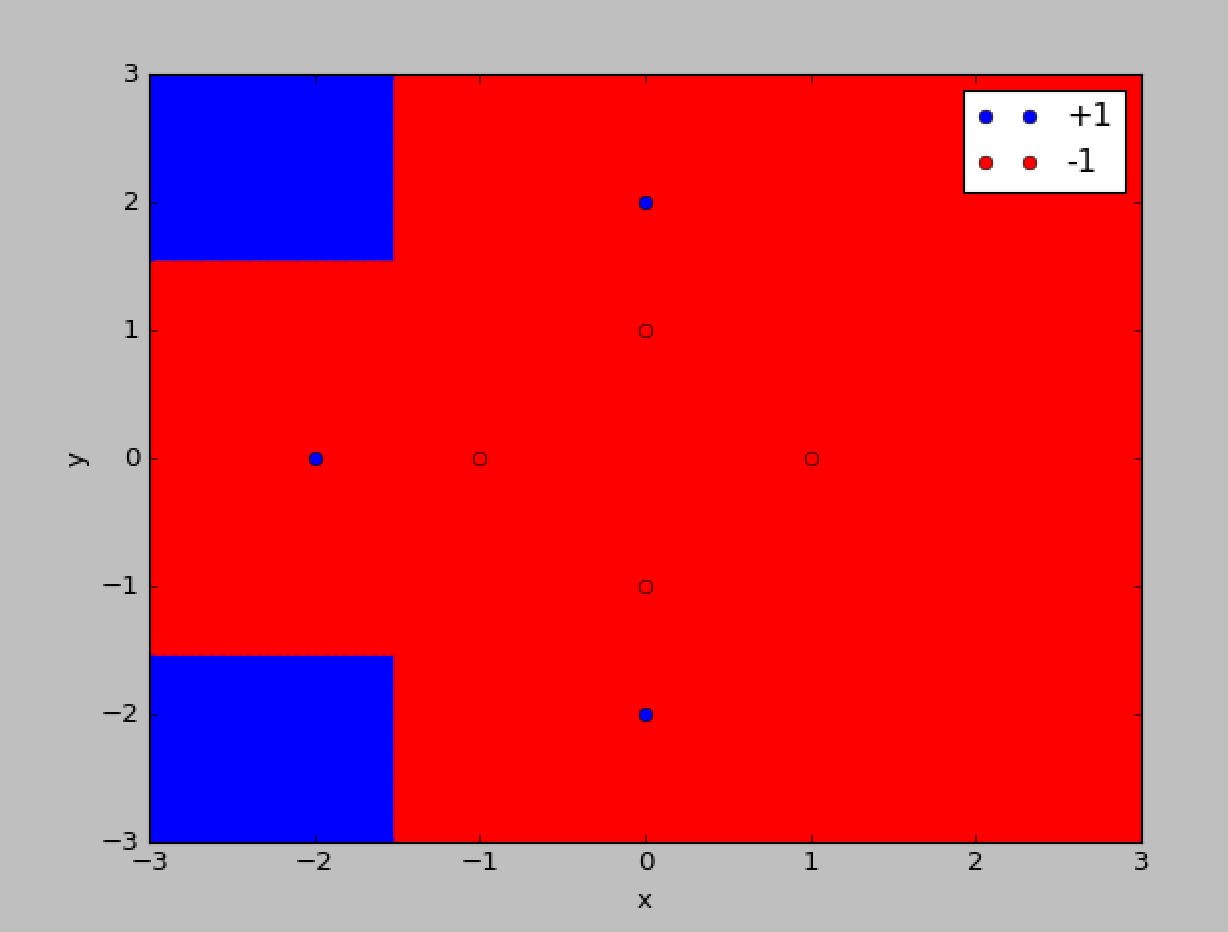
\includegraphics[scale=0.6]{6-1a2.png}
	\item Below is the 1-NN decision boundaries after the transform is performed.
	
	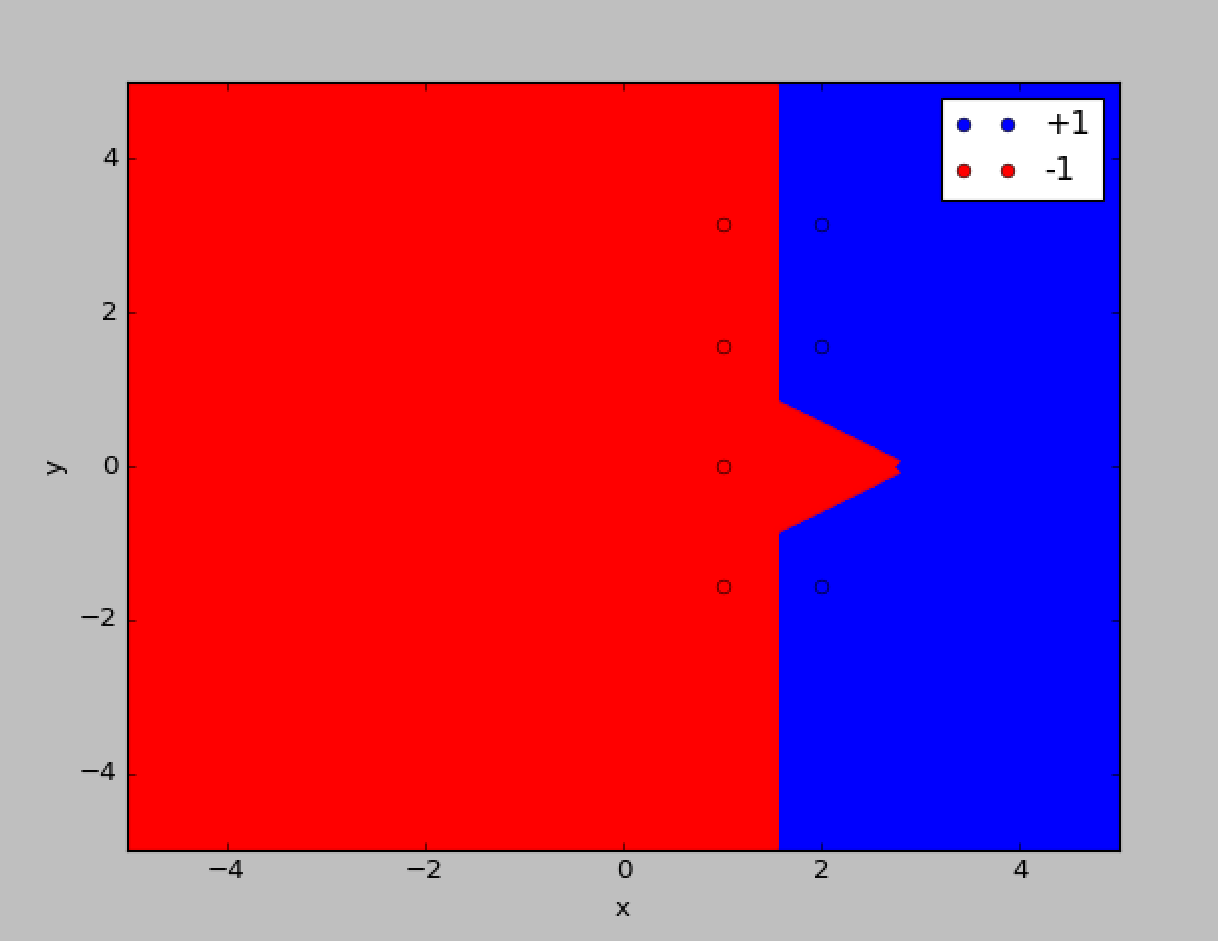
\includegraphics[scale=0.6]{6-1b1.png}
	
	Similarly, here are the boundaries for 3-NN.
	
	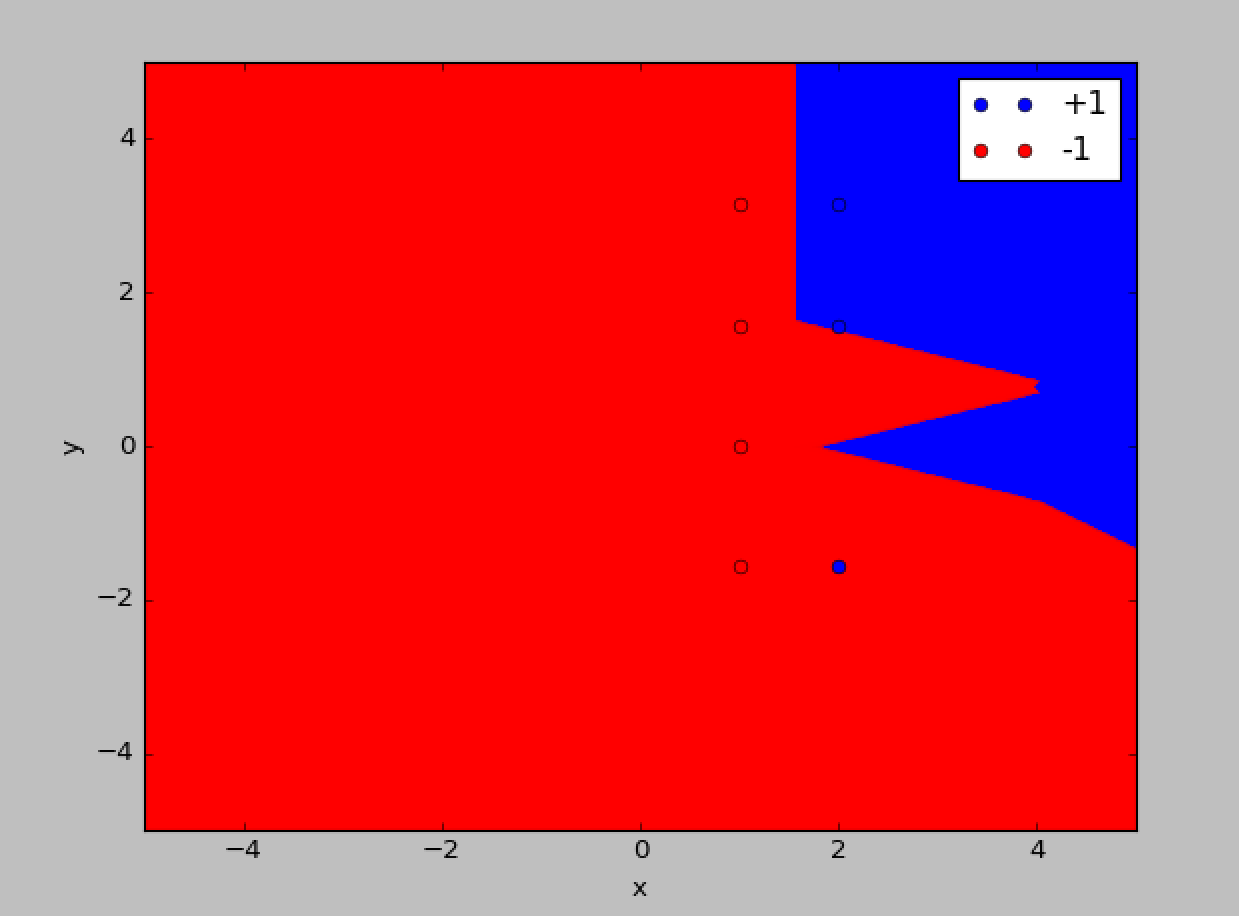
\includegraphics[scale=0.6]{6-1b2.png}
\end{enumerate}

\section*{Problem 6.4}
\begin{enumerate}[label=(\alph*)]
	\item Below is the graph for 1-NN for the decision boundaries of the points we gathered in Problem 3.1
	
	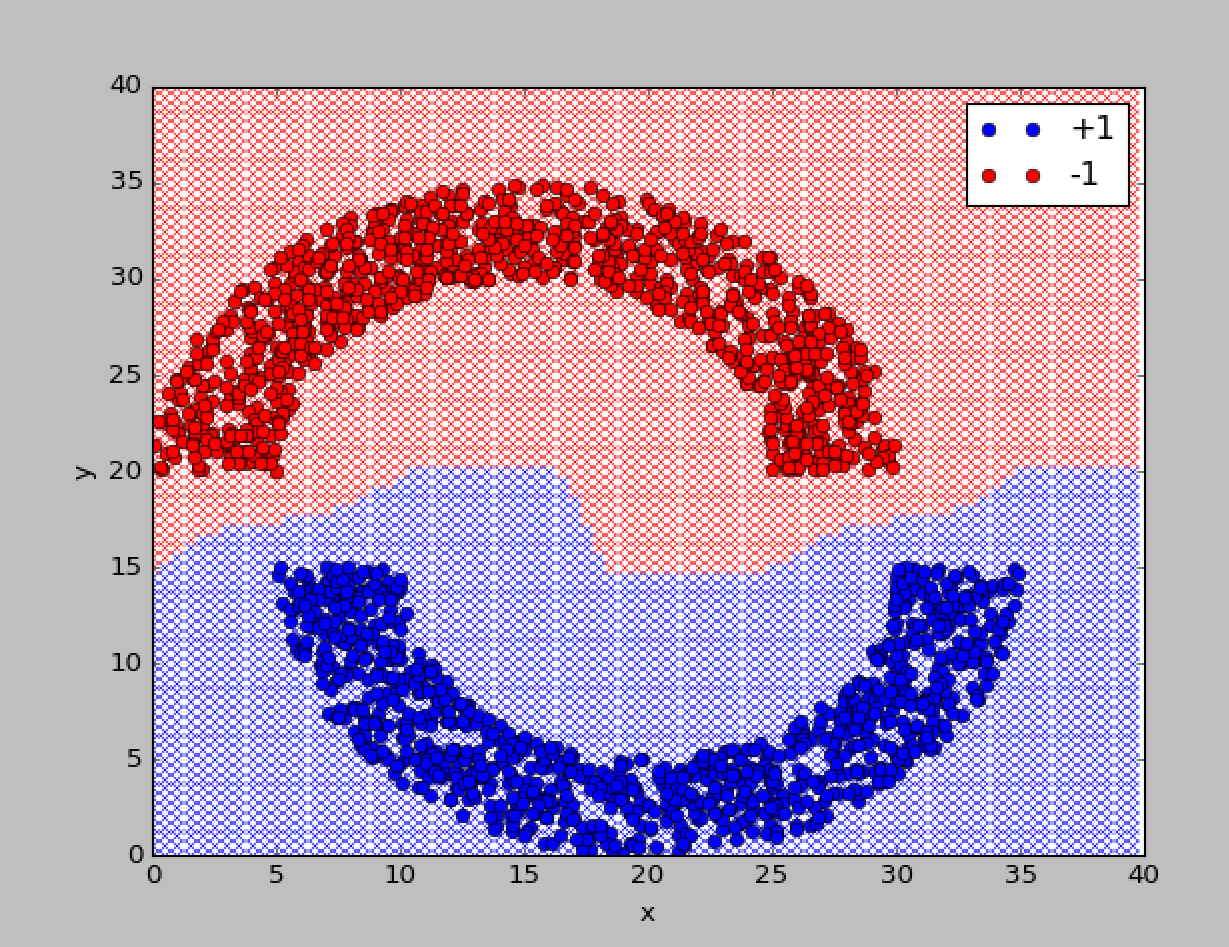
\includegraphics[scale=0.6]{6-4-1.png}
	
	Similarly, here is the graph for 3-NN for the same points. There is very marginal difference but the gains are huge in the VC-boundaries. (The biggest noticeable difference is on the left hand side, which is a little rockier with the 3-points)
	
	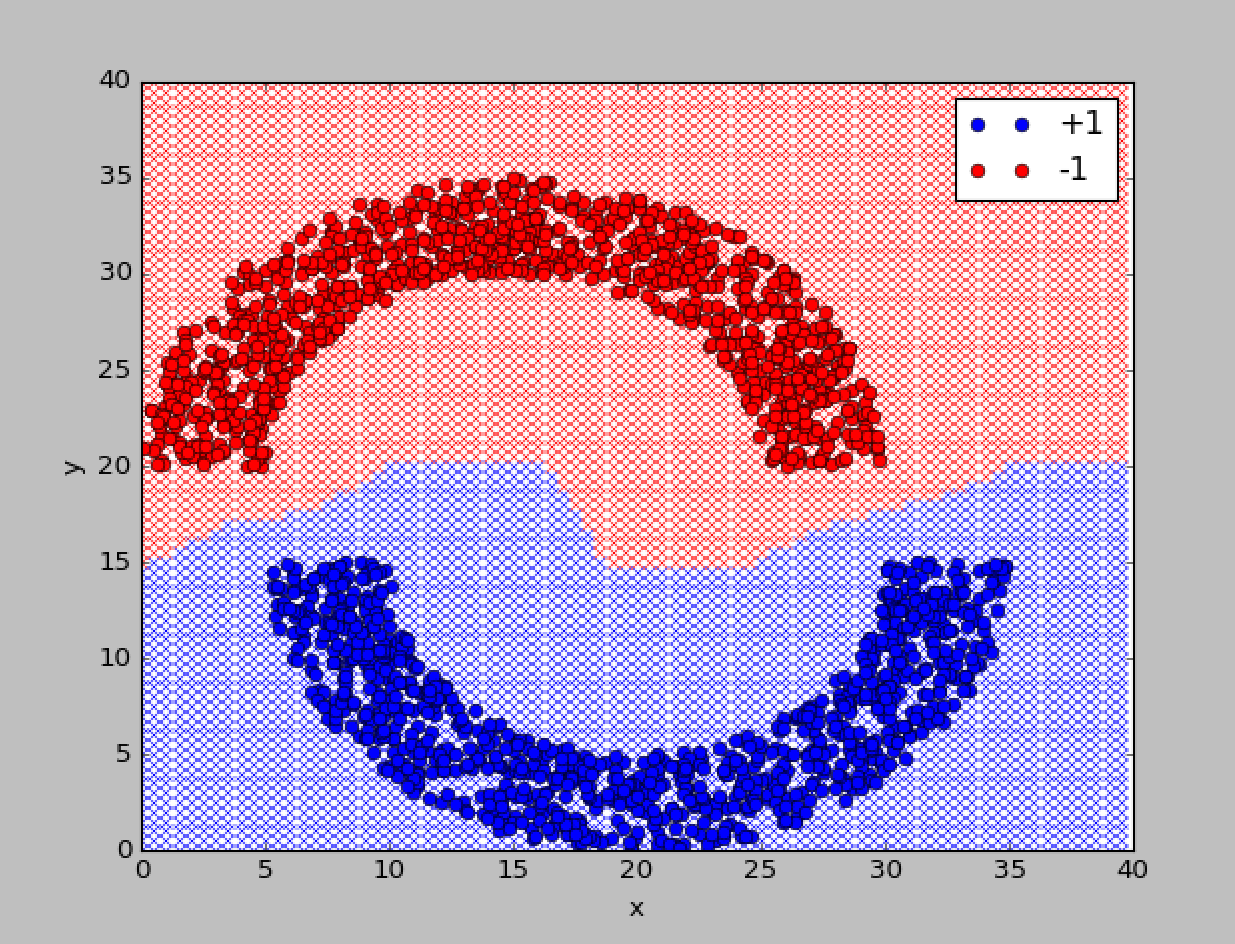
\includegraphics[scale=0.6]{6-4-2.png}
\end{enumerate}

\section*{Problem 6.16}
\begin{enumerate}[label=(\alph*)]
	\item After running the two algorithms on the randomly generated data, I got a run-time of \textbf{668.27 seconds} for the brute-force and a run-time of \textbf{145.25 seconds} for the branch and bound algorithm. Branch and bound allows us to disregard a large number of points (due to being able to ignore whole clusters) for a majority of the calculations. This cuts own significantly on run-time.
	\item With the gaussian generated data, I got a run-time of \textbf{701.22 seconds} for the brute-force and a run-time of \textbf{551.27 seconds} for the branch and bound algorithm.
	\item When the points aren't completely randomly thrown about, it becomes harder to use the clustering algorithm to improve performance. For instance, the following picture shows the distributions of the points within the clusters when the points are determined from Gaussians:
	
	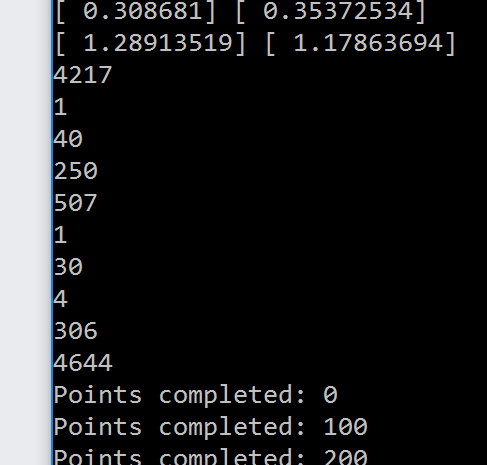
\includegraphics[scale=0.6]{6-16-1.png}
	
	As you can see, most of the points find themselves in one of two clusters. The two main clusters therefore end up having large radii. Each nearest neighbor calculation then ends up requiring checking the majority of the points anyway. This somewhat defeats the purpose of the whole optimization in the first place.
	\item It is not the number of points that should decide whether you use branch and bound or not, but rather how the points are distributed and how spread out you can expect them to be. If they are all going to end up in a couple clusters, you'll need either very precise center picks (the greedy algo may not suffice) or a lot more optimization.
\end{enumerate}

\end{document}